Performing complex operations on battery-less energy harvesting embedded platforms is challenging from many points of view. Here we shall briefly provide a background on computation with energy harvesting embedded systems. 

\subsection{Energy Harvesting: Background}
\label{sec:background_harvesting}

Supplying power to tiny embedded computers using batteries alone is not sustainable. European Commission estimates that more than 160 kilotons of consumer batteries enter the European Union annually~\cite{eu_batteries_2016}. Since not all batteries are recycled, they constitute a potential environmental hazard. A potent solution is to replace batteries with smaller, but environment friendly {(super-)capacitors} (promising millions of charge/discharge cycles~\cite[Sec. I]{ongaro_pwre_2012}) and to supply them {\em directly from the ambient energy sources}---creating a truly self-sustainable computing device. The limitation of the capacitor as a storage device is energy density that is inferior to a battery, making effective capacitor discharge times orders of magnitude smaller than for a battery.

Given current technology development, battery-less systems are best suited for very long-term sensing and monitoring where access to recharge is either prohibitive or impossible. These include battery-less image capture and processing~\cite{naderiparizi_rfid_2015}, animal monitoring~\cite{thomas_jbcs_2012} or implantable~\cite{rodriguez_tbcs_2015} and digestible~\cite{nadeau_naturebio_2017} sensors.

Many platforms enable intermittent, battery-less computation. For instance, computation RFIDs---open-source TI MSP430-based~\cite{wolverine} WISP~\cite{wisp5} (with its variants such as WISPCam~\cite{naderiparizi_rfid_2015}, NFC-WISP~\cite{zhao_rfid_2015} or NeuralWISP~\cite{holleman_biocas_2008}), Moo~\cite{moo}, and commercial ones such as~\cite{medusa_farsens_2017}. Other intermittently-powered platforms include ambient backscatter tag~\cite{liu_sigcomm_2013,parks_sigcomm_2014} or battery-less phone~\cite{talla_imwut_2017}. In all of the above, the main source of energy harvested is the electromagnetic radiation in the radio frequency range (ambient transmitters such as high power TV transmitters~\cite{liu_sigcomm_2013} or dedicated RFID antenna~\cite{wisp5,moo,talla_imwut_2017,medusa_farsens_2017,holleman_biocas_2008,naderiparizi_rfid_2015}). Naturally, other forms of energy harvesting sources exist, including temperature gradient, (micro-)motions, light/sun radiation, vibrations, and body fluid flow (blood, gastric acid). The reader is referred to example extensive surveys discussing energy harvesting for low-power embedded systems~\cite{paradiso_pvc_2005,soyata_csm_2016,prasad_comst_2014,ku_cst_2016}.

\begin{table}
	\centering
	\begin{tabular}{|c|c|}
	\hline
	Platform name & Storage capacitor size \\
	\hline \hline
	Moo~\cite{moo} & 0.1\,F \\
	WISPCam~\cite{naderiparizi_rfid_2015} & 6.08\,mF \\ %tested [11.24, 17.45, 21.98]\,mF
	NFC-WISP~\cite{zhao_rfid_2015} & 300\,$\mu$F \\
	NeuralWISP~\cite{holleman_biocas_2008} & 100\,$\mu$F \\
	WISP~\cite{wisp5} & 47\,$\mu$F \\
	{\em BioImpedance} sensor~\cite{rodriguez_tbcs_2015} & 20\,$\mu$F \\
	{\em Ingestible} sensor~\cite{nadeau_naturebio_2017} & 220\,$\mu$F\\
	\hline
	\end{tabular} 
\caption{Comparison of {\em default} energy storage sizes for various battery-less platforms. Observe a huge variation in storage capacity. We note that values for other representative platforms~\cite{medusa_farsens_2017,talla_imwut_2017,liu_sigcomm_2013,parks_sigcomm_2014} were not reported in their respective papers.}
\label{table:capacitor}
\end{table}

The biggest technical problem with energy provided from the ambient to battery-less platforms is that harvested energy is not stable and difficult to predict accurately. Combined with the fact that energy supply is small, there is little leeway to store enough of energy to guarantee prolonged periods of computation. Energy breaks happen every hundred of milliseconds, refer again to e.g.~\cite[Fig. 1]{mementos}. This causes each program running on such platform to restart. Solution to the problem is to divide the program into smaller parts that guarantee execution within a discharge region and track the state of the program in-between execution times.

\subsection{Memory Consistency}
\label{sec:background_consistency}

Naturally, content of a volatile memory (i.e. run-time stack, global and local variables) of the microcontroller and program registers are erased after each power failure. Only what resides in a non-volatile memory, e.g. FRAM, persists after system reboot. A solution to sustain the progress of the program from the last power failure, instead from the beginning (the \emph{Sisyphus} effect~\cite[Sec. 2]{mementos})is a periodic checkpointing of a program state~\cite{mementos,hibernusplusplus,quickrecall,idetic}. The periodicity, and a position of a checkpoint, is the core of the contribution behind each of the proposed checkpoining solution. 

\begin{figure}
	\centering
	\subfloat[Simplified C code snippet of a CRC calculation from~\cite{hicks_mibench2_2016}: per-byte message division by a polynomial; \texttt{NV} denotes non-volatile variable declaration]{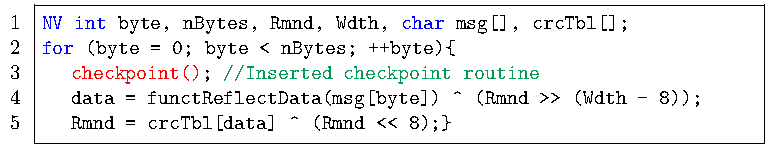
\includegraphics[width=\columnwidth]{figures/crc_example}\label{fig:crc_example}}\\
	\subfloat[Consecutive execution steps of the loop body in the snippet above: non-volatile checkpointing did not guarantee data consistency as data has been manipulated (line 10) with stale reminder (line 3)]{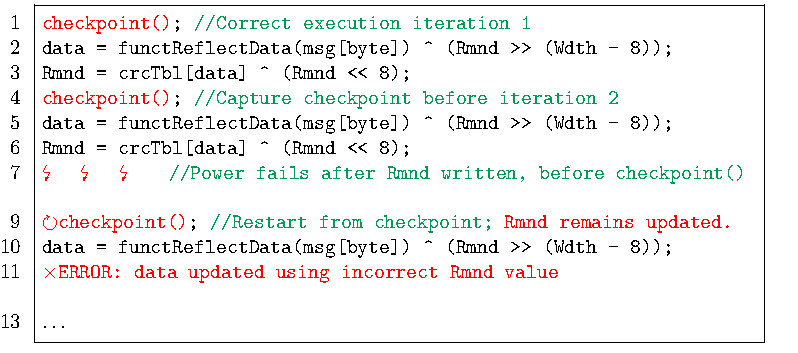
\includegraphics[width=\columnwidth]{figures/crc_example_war}\label{fig:crc_example_war}}
	\caption{Code example demonstrating effect of write after read on volatile memory checkpointing.}
	\label{fig:code_demo_incosistency}
\end{figure}

Nevertheless, regular checkpointing of program state to a non-volatile memory still does not guarantee consistency. This phenomenon has been discussed extensively in e.g.~\cite{chain,alpaca}. For the completeness of this exposition we will provide our own example demonstrating this problem. For this please refer to Fig.~\ref{fig:code_demo_incosistency} and compare with~\cite[Sec 2.3]{alpaca},~\cite[Sec. 2.1]{chain}. We take an example of a fast procedure to calculate cyclic redundancy check (CRC) from~\cite{hicks_mibench2_2016}. Therein a CRC must be calculated for $\texttt{nBytes}$-long message $\texttt{msg}$ with specified initial reminder $\texttt{Rmnd}$ and constant, $\texttt{Rmnd}$ variable type-dependent, $\texttt{Wdth}$. Despite regular, fixed position checkpoints (line 3 in Fig.~\ref{fig:crc_example}) of all variables which are declared as non-volatile (denoted as \texttt{NV}) variable $\texttt{data}$ is calculated incorrectly. This is because of a write after read (WAR) hazard of variable $\texttt{Rmnd}$. WAR hazard is caused by consecutive write and read in-between two consecutive checkpoints using $\texttt{checkpoint()}$ function: $\texttt{data}$ variable is written \emph{before} (line 10 in Fig.~\ref{fig:crc_example_war}) $\texttt{Rmnd}$ is read (line 6 in Fig.~\ref{fig:crc_example_war}), or more specifically---updated before a new execution loop. 

\subsection{Assumption on the Type of Computing Hardware}
\label{sec:background_hardware}

We assume that we operate on the microcontroller (more generally, computing hardware) equipped with a mix of volatile and non-volatile memory, such as FLASH, Ferroelectric RAM or Magnetoresistive RAM. \sys does not assume to rely on specific memory type (either volatile or non-volatile), in contrary to earlier works targeting non-volatile processors~\cite{su_date_2017,ratchet,quickrecall,nvp}. Actually, \sys will exploit the properties of both memory types to maximize performance metrics of the program being executed. We make \sys able to I/O operations, however we do not enable the scheduling of operations (which \emph{nota bene} forms a foundation for a simple runtime). All in all, our hardware model follows in assumptions the two most relevant intermittently-powered execution environments~\cite{alpaca,chain}.

\subsection{(Task-based) Intermittent Computing: Background}

There is increasing amount of work that deals with protecting memory consistency. Table~\ref{table:chechpoint_comparison} provides a summary of various costs associated with most relevant task-based/checkpointing solutions. This table generalizes discussion from~\cite[Sec. 2.4]{alpaca}.

\begin{table}
	\centering
	\begin{tabular}{|c|c|c|c|}
		\hline
		{~} & CP & SZ & NV \\
		\hline\hline
		\!\!Mementos~\cite{mementos}\!\! & \!\!$N_2\leq N_1$\!\! & \!\!R + S\!\! & \!\!R + S\!\! \\
		\!\!DINO~\cite{dino}\!\! & $N_2$\!\! & \!\!R + W\!\! & \!\!R + W\!\! \\
		\!\!Chain~\cite{chain}, Alpaca~\cite{alpaca}\!\! & \!\!$N_2$\!\! & P\!\! & \!\!2W + P\!\!\\
		\!\!Ratchet~\cite{ratchet}, Clank~\cite{hicks_isca_2017}\!\! & $N_3\geq N_2\geq N_1$\!\! & \!\!R\!\! & R\!\!\\
		\hline 
	\end{tabular}
	\caption{Cost of various checkpointing methods; Symbols---R: register, S: stack, W: WAR-dependent variables, P: program counter, $N_1, N_2, N_3$: relative number of checkpoints for each method, CP: no. checkpoints, SZ: checkpoint size, NV: copy to non-volatile memory size.}
	\label{table:chechpoint_comparison}
\end{table}

The energy cost of a single checkpoint is $w\text{CP(SZ+NV)}$, where $w$ is the cost of a single word copy into a non-volatile memory. Decrease of CP decreases the energy cost associated with each state preservation method and reduces operation cost which in most simplistic terms is defined as $\mathcal{O}(\text{CP})+\mathcal{O}(\text{PL})$, where PL is the cost of program execution without checkpointing. On the other hand, this increases task/checkpoint re-execution time. 

Moreover, each battery-less platform has different storage sizes, refer to Table~\ref{table:capacitor}, which causes different charge/discharge periods. This result in different execution times. In the worst case the size of the capacitor might be too small to execute one task written by the programmer.

%prior systems do fine grained task division (virtualization) {clank,aplaca}

Task is a programmer (or compiler) defined code that is executed based on consistent set of inputs, i.e. memory fetched from a specified memory location, producing a consistent output stored in a specified (the same or different) memory location. Syntactically, we can treat a task as a continuous sub-section of a large program encapsulated by (i) task specific keywords defining the beginning and the end of a task and (ii) message passing between tasks connected with each other.

\begin{figure}
	\centering
	%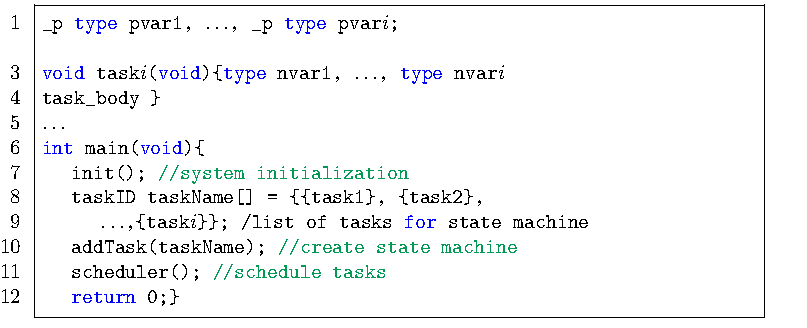
\includegraphics[width=\columnwidth]{figures/taskification_example}
	\caption{Task flow example executed by \sys.\todo{Draw an example task diagram}{Przemek}}
	\label{fig:task_flow_example}
\end{figure}

Let us look into how task-based programming is performed relying on an example provided in Fig.~\ref{fig:task_flow_example}. Each task is uniquely identified by a keyword. A separate part of code specifies a state machine than governs how tasks are connected with each other. This way a programmer specifies to which other task a current task needs to pass the result of its computation (and it can be either a new task or the task itself). Tasks are executed atomically. That is, task will be executed only once and will be considered as completed only when a task reaches a final instruction line informing a scheduler that a program is ready to enter into a new task.

Just like Chain~\cite{chain} and Alpaca~\cite{alpaca}, \sys does not support concurrent programming, multi-threading (multi-task sequence) and does not consider priorities and on-demand scheduling. These features are extremely important to consider but go beyond the scope of this work. A comparative description of \sys is given in Table~\ref{table:feature_comparison}. 

Important and a strong assumption about task-based programming for intermittently-powered systems is that an energy availability for the largest possible task execution must be guaranteed. Task is an atomic operation and  must preserve execution order and memory manipulations. Task that follows such an assumption is equivalent to task being executed on a continuously-powered non-interrupted system. Whenever a task cannot fit into a single energy reservoir, it must be divided into tasks that will be executed within a single discharge cycle.

\begin{table}
	\begin{tabular}{|c|c|c|c|}
		\hline
		{~} & Alpaca~\cite{alpaca} & Chain~\cite{chain} & This work \\
		\hline\hline
		Task connections & in-task & in-task & outside \\
		Task re-use & N & N & Y\\
		Memory model & globals & globals & globals\\
		Concurrency & N & N & N \\
		Task blocking & N & N & Y \\
		Energy-adaptive & N & N & Y \\
		\hline
	\end{tabular}
	\caption{Comparison of existing task-based execution models against \sys.}
	\label{table:feature_comparison}
\end{table}

\todo{Elaborate on the ``key challenge'' paragraphs near the end of the intro}{Przemek}

%%%Notes%%%

%We can write the problem of maximizing all task sizes formally as
%
%\begin{equation}
%\underset{i}{\arg\,\max} \sum_{i}m_i+t_i \text{~subject to~} \forall_i mi+t_i>e,
%\end{equation}
%
%where $e$ is the required minimum energy to perform a task, $i$ is the total number of tasks, $m_i$ and $t_i$ are the cost of task traversal (memory copying time of task variables) and time to complete one task, respectively.

%Two problems with fixed-size task in intermittent execution. (a) task underestimation: task executed at device with capacitor size $X$, will not execute at device with capacitor $X\gg Y$; (b) task overestimation: with stable energy source task tracking causes unnecessary overhead.

%\begin{figure}
%\centering
%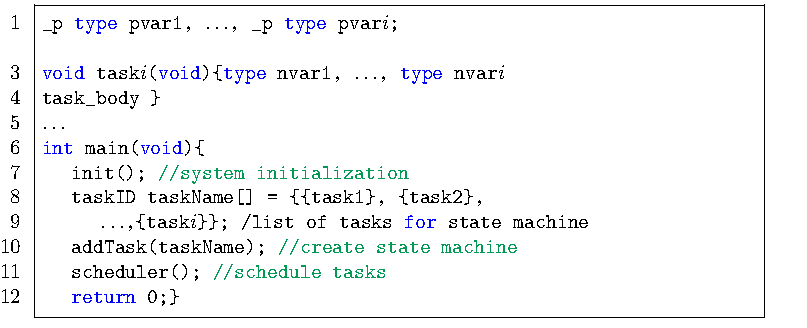
\includegraphics[width=\columnwidth]{figures/taskification_example}
%\caption{Program divided into tasks.}
%\label{fig:taskification_example}
%\end{figure}

%Other forms of intermittent platforms will share the same problem. One of them considers actuation platforms, which will be powered directly from energy harvesting sources~\cite{}. will share the energy storage with computing platform. However, power supply for actuators is order of magnitude larger than for computation. Therefore, although capacitor is large enough to perform computation alone, energy to power actuators takes precedence leaving not much space for computing.